\chapter[Experiments of platooning concept in traffic simulator]{Experiments of platooning concept in traffic simulator\chaptermark{Experiments of platooning concept}}
\chaptermark{Experiments of platooning concept}

This chapter covers testing of platooning concept in our developed traffic simulator (see Chapter 4). By parameters which are mentioned in Section 4.2.2 and by the selection of the highway type we simulated and checked positive effects of platooning concept on highway traffic. Later in this chapter there are descriptions and commentaries of several tests and simulations that correspond to the maximum and real utilisation of highway. We simulated 3 types of highway – one, two and three-lane highway – and length of highway segments is 5 km.

The main feature of traffic which we studied and compared was maximum capacity of highway and average speed of passenger vehicles. Because of long duration (12 minutes) of tests, we were not able to do more than two times and do statistical calculations of these features. Instead of that we used a value at which the capacity of simulator stabilized as maximum capacity and average speed of passenger vehicles during last 10 minutes of test (2 minutes to fill the simulation environment).








\section[Experiment \#1: Maximum capacity of lane in simulator]{Experiment \#1: Maximum capacity of lane in simulator\sectionmark{Experiment \#1...}}
\sectionmark{Experiment \#1...}

In this experiment we tried to find out maximum capacity of one highway lane in our simulator with different ratio between platooning and non-platooning passenger vehicles. Because we used very similar preconditions, we expected very similar results to the theoretical example which is described in Section 2.5. In order to confirm this assumption we compared results only for percentage of platooning vehicles equal to 0\% and 100\%, because the Equation \ref{eq:max_cap_platooning} is not defined for more values.





\subsection*{Simulator setting for the test}
\begin{itemize}
\item Average speed: 25 m/s, 30 m/s, 35 m/s
\item Speed dispersion: 0 m/s
\item Length of platoon: 6
\item Number of lanes:  1
\item Platooning vehicles ratio: 0\%, 20\%, 40\%, 60\%, 80\%, 100\%
\item Generation limit: false
\item Generate trucks: false
\end{itemize}



\subsection*{Experiment result}

In Figure \ref{fig:5_1-1} and Table \ref{tab:5_1-1} you can see dependency of maximum capacity of lane and percentages of platooning vehicles. The maximum capacity is a nonlinear dependence on percentage of platooning vehicles. 

\begin{figure}[ph]
\centering
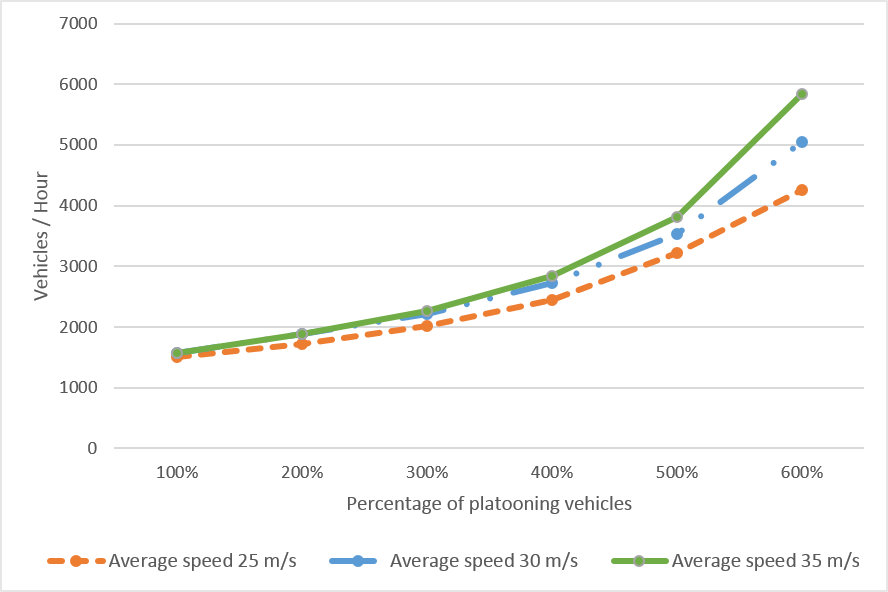
\includegraphics[width=0.82\textwidth,height=0.82\textheight,keepaspectratio]{figures/Chapter_5/5_maximum_cap.png}
\centering
\protect\caption[Maximum capacity of one lane for 25 m/s, 30 m/s, 35 m/s]{\label{fig:5_1-1}Maximum capacity of one lane for 25 m/s, 30 m/s, 35 m/s - capacity measured only for 0\%, 20\%, 40\%, 60\%, 80\%, 100\% platooning vehicles, so as to be more visual the line connecting measured data was added}
\end{figure}

\begin{table}[ph]
\begin{centering}
\begin{tabular}{|c|c|c|c|c|c|c|}
\hline 
Average speed / Platooning \% &	0\% &	20\% &	40\% &	60\% &	80\% &	100\%\tabularnewline
\hline 
25 m/s &	1 575 &	1 839 &	2 190 &	2 725 &	3 513 &	5 015\tabularnewline
\hline 
30 m/s &	1 504 &	1 760 &	2 116 &	2 701 &	3 528 &	5 408\tabularnewline
\hline 
35 m/s &	1 566 &	1 852  & 2 224 &	2 825 &	3 814 &	5 832\tabularnewline
\hline 
\end{tabular}
\centering
\protect\caption{\label{tab:5_1-1}Measured values of maximum capacity of lane for different average speed}
\end{centering}
\end{table}

We expected that our maximum capacity of lane results from simulator should have been similar to calculated values which we got by solving Equation \ref{eq:max_cap_platooning}. In Tables \ref{tab:5_1-2}, \ref{tab:5_1-3} there are comparisons of the calculated Theoretical maximum capacity of lane and of our adequate reached values from Table \ref{tab:5_1-1}. 

\begin{table}[ht]
\begin{centering}
\begin{tabular}{|c|c|c|c|}
\hline 
Experiment / & 	Simulator 0\%  & 	Theoretical 0\%   &	Ratio  \tabularnewline
 Maximum lane & 	 platooning & 	  platooning  &	 (Reached / \tabularnewline
 capacity& 	  vehicles & vehicles & Theoretical)\tabularnewline
\hline 
Average speed 25 m/s &	1 575 &	1 666 &	94.54\%\tabularnewline
\hline 
Average speed 30 m/s &	1 524 &	1 688 &	90.31\%\tabularnewline
\hline 
Average speed 35 m/s &	1 566 &	1 702 &	92.01\%\tabularnewline
\hline 
\end{tabular}
\centering
\protect\caption{\label{tab:5_1-2}Comparison of maximum reached value and maximum theoretical values of maximum lane capacity for 0\% platooning vehicles}
\end{centering}
\end{table}

\begin{table}[ht]
\begin{centering}
\begin{tabular}{|c|c|c|c|}
\hline 
Experiment /  & Simulator 100\% & 	Theoretical 100\%   &	Ratio \tabularnewline
 Maximum lane &  platooning  & 	 platooning  &	 (Reached / \tabularnewline
 capacity& vehicles & 	 vehicles &	 Theoretical)\tabularnewline
\hline 
Average speed 25 m/s & 5 015 &	5 129 &	97.78\%\tabularnewline
\hline 
Average speed 30 m/s & 	5 408 &	5 684 &	95.14\%\tabularnewline
\hline 
Average speed 35 m/s&	5 842 &	6 097 &	95.82\%\tabularnewline
\hline 
\end{tabular}
\centering
\protect\caption{\label{tab:5_1-3}Comparison of maximum reached value and maximum theoretical values of maximum lane capacity for 100\% platooning vehicles}
\end{centering}
\end{table}

All our reached values for 0\% platooning vehicles are up to 10\% less than the theoretical ones. It is caused by our different approach to safe distance which should be in front of the vehicle. In our case the Front safe distance to vehicle of the same speed consists of \textit{Reaction distance} and \textit{Safe time distance}. The example does not count with the \textit{Reaction distance}. It is also influenced by changing speed of vehicles which oscillate around optimal distance to a front vehicle. The reached values for 100\% platooning have smaller percentage mistake up to 5\%, because the \textit{Reaction distance} is contained in Front safe distance, which effects only the leading vehicles of each platoon. 

We think that this less than 10\% difference proves that the simulator can be used for testing of maximum capacity of highway with platooning concept.

For other next experiments we used simulation with an average speed, zero speed dispersion, constant platooning length, no generation limit and no trucks as a reference value for maximum capacity of a lane and the average speed over different percentage of platooning vehicles.

















\newpage

\section[Experiment \#2: Linear dependency of maximum highway capacity on number of its lanes]{Experiment \#2: Linear dependency of maximum highway capacity on number of its lanes\sectionmark{Experiment \#2...}}
\sectionmark{Experiment \#2...}

We wanted to verify whether the maximum capacity is proportional to number of lanes with overtaking. We expected the proportionality, because number of overtaking and changing lanes actions will be very low thanks to \textit{Speed dispersion} = 0. We tried to prove it by comparison of multiplies of one-lane highway capacity with two-lane highway capacity and three-lane highway capacity.







\subsection*{Simulator setting for the test}
\begin{itemize}
\item Average speed: 30 m/s
\item Speed dispersion: 0 m/s
\item Length of platoon: 6
\item Number of lanes:  1, 2, 3
\item Platooning vehicles ratio: 0\%, 20\%, 40\%, 60\%, 80\%, 100\%
\item Generation limit: false
\item Generate trucks: false
\end{itemize}



\subsection*{Experiment result}

In Table \ref{tab:5_2-1} there are results of maximum capacity of highway with different numbers of lanes and with different percentage of platooning vehicles. All generated vehicles had the same speed. In the next Table \ref{tab:5_2-2} there is percentage comparison of maximum capacity of two-lane and three-lane highway with adequate multiple of maximum capacity of one-lane highway. Since the maximum capacity of multi-lane highways is almost always smaller than multiplies of the one-lane highway, the maximum capacity of highway in our simulator is not exactly proportioned to the number of lanes, but it is very close to it.

\begin{table}[ht]
\begin{centering}
\begin{tabular}{|c|c|c|c|c|c|c|}
\hline 
Type / Platooning \% &	0\% &	20\% &	40\% &	60\% &	80\% &	100\%\tabularnewline
\hline 
1 lane highway &	1 504 &	1 760 &	2 116 &	2 701 &	3 528 &	5 408\tabularnewline
\hline 
2 lane highway &	3 015 &	3 552 &	4 214 &	5 218 &	7 016 &	10 290\tabularnewline
\hline 
3 lane highway &	4 462 &	5 186 &	6 250 &	7 748 &	10 285 &	15 034\tabularnewline
\hline 
\end{tabular}
\centering
\protect\caption{\label{tab:5_2-1}Measured maximum capacity of highway with 1, 2 and 3 lanes for percentage of platooning vehicles}
\end{centering}
\end{table}

\begin{table}[ht]
\begin{centering}
\begin{tabular}{|c|c|c|c|c|c|c|}
\hline 
Ratio / Platooning \% &	0\% &	20\% &	40\% &	60\% &	80\% &	100\%\tabularnewline
\hline 
2 lane highway &	1.0017 &	1.0090 &	0.9956 &	0.9658 &	0.9942 &	0.9514\tabularnewline
/ triple of 1 lane highway & & & & & &\tabularnewline
\hline 
3 lane highway &	0.9883 &	0.9821 &	0.9844 &	0.9560 &	0.9716 &	0.9267\tabularnewline
/ triple of 1 lane highway & & & & & &\tabularnewline
\hline 
\end{tabular}
\centering
\protect\caption{\label{tab:5_2-2}Ratio of multi-lanes highways maximum capacities and adequate multiple of maximum capacity of one lane highway}
\end{centering}
\end{table}



















\section[Experiment \#3: Maximum capacity of two lane highway with real traffic conditions of Czech Republic]{Experiment \#3: Maximum capacity of two lane highway with real traffic conditions of Czech Republic\sectionmark{Experiment \#3...}}
\sectionmark{Experiment \#3...}


In real situation all vehicles would never travel by  the same speed level. So this experiment is focused on effects of platooning concept in Czech highway environment with the speed based on research which is mentioned in Chapter 2. We set main parameters of our simulator (Chapter 4) and we run the simulation of highway of length 5 km for 15 minutes to find out, how the traffic would behave for different percentage of platooning vehicles. 

We expected positive effect on maximum capacity of highway and negative effect on average speed of passenger vehicles, because long platoon of slower vehicles should more slow down the lane and because the overtaking vehicles have to overtake long platoons for longer time too. 






\subsection*{Simulator setting for the test}

\begin{itemize}
\item Average speed: 34 m/s
\item Speed dispersion: 3 m/s
\item Length of platoon: 2-6
\item Number of lanes:  2
\item Platooning vehicles ratio: 0\%, 20\%, 40\%, 60\%, 80\%, 100\%
\item Generation limit: false
\item Generate trucks: false, true
\item Percentage of passenger vehicles in traffic: 65\%
\item Overtaking: Snake type
\end{itemize}

\subsection*{Experiment results}

We did simulations with traffic in two-lane highway without truck traffic (see maximum reached capacity during time in Figure \ref{fig:5_3-1}) and with included truck traffic (See level of maximum reached capacity during time in Figure \ref{fig:5_3-2}).

\begin{figure}[ph]
\centering
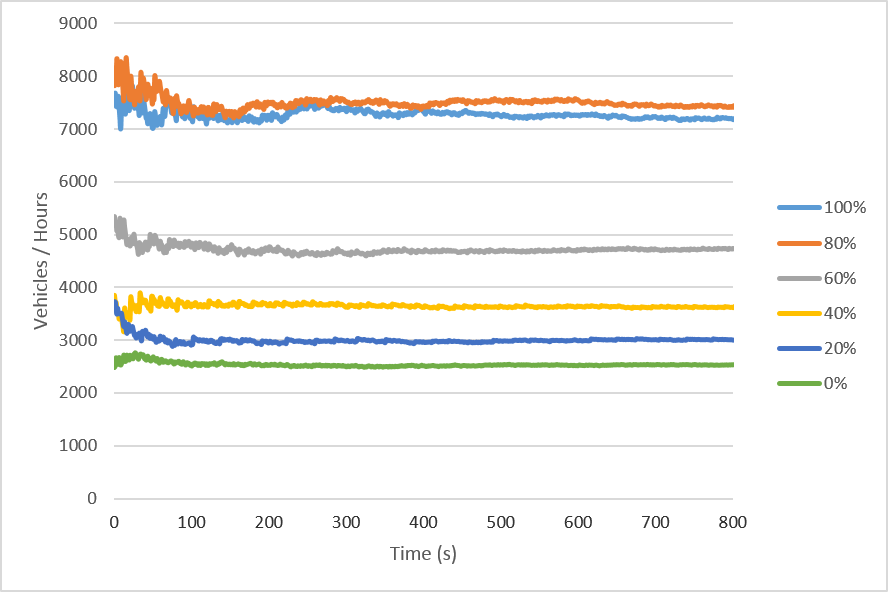
\includegraphics[width=0.82\textwidth,height=0.82\textheight,keepaspectratio]{figures/Chapter_5/5_max_2lane_Ntrucks.png}
\centering
\protect\caption[Maximum capacity of two-lane highway and real traffic conditions without trucks]{\label{fig:5_3-1}Maximum capacity of two-lane highway and real traffic conditions without trucks}
\end{figure}



\begin{figure}[ph]
\centering
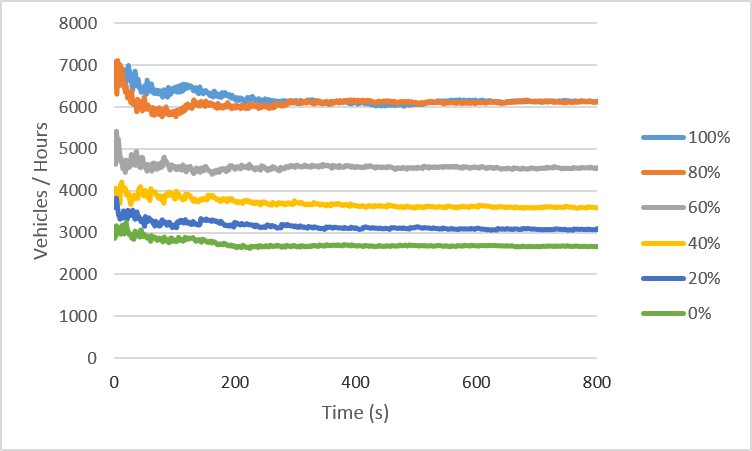
\includegraphics[width=0.82\textwidth,height=0.82\textheight,keepaspectratio]{figures/Chapter_5/5_max_2lane_trucks.png}
\centering
\protect\caption[Maximum capacity of two-lane highway and real conditions with trucks]{\label{fig:5_3-2}Maximum capacity of two-lane highway and real conditions with trucks}
\end{figure}



As we expected, in Figure \ref{fig:5_3-4} we can see positive effect of platooning concept on maximum capacity of two-lane highway with realistic conditions. 

This confirmed our assumption that there is some relation between percentage of platooning vehicles and the average speed during maximum usage of highway. There is a tendency that the average speed is decreasing with increasing percentage of platooning vehicles, this can be seen in Figure \ref{fig:5_3-3}.

\begin{figure}[ph]
\centering
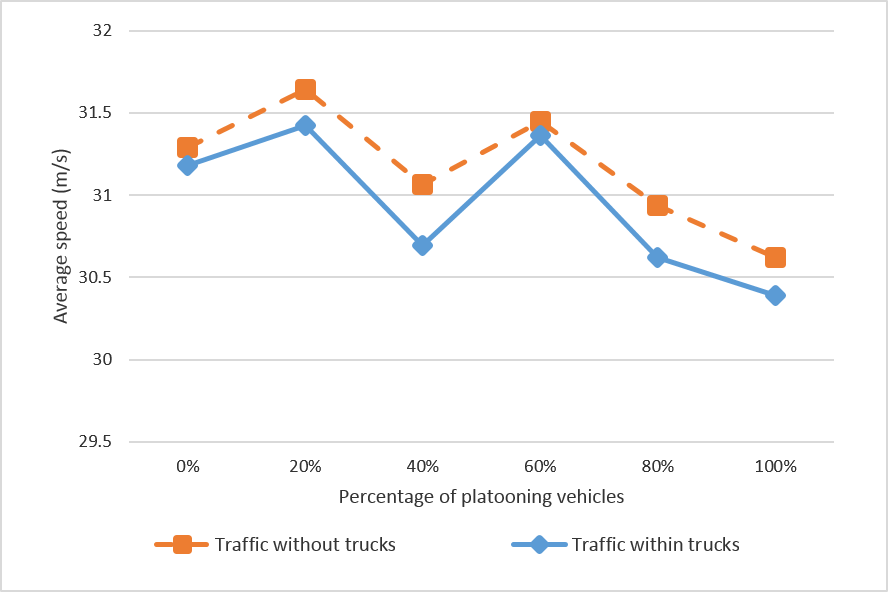
\includegraphics[width=0.82\textwidth,height=0.82\textheight,keepaspectratio]{figures/Chapter_5/5_E3_avgSpeed.png}
\centering
\protect\caption[Average speed of traffic without and with trucks in two-lane highway]{\label{fig:5_3-3}Average speed of traffic without and with trucks in two-lane highway  - average speed measured after stabilization of traffic and only for 0\%, 20\%, 40\%, 60\%, 80\%, 100\% platooning vehicles, so as to be more visual the line connecting measured data was added.}
\end{figure}

As it can be seen in both tests, maximum capacity (Figure \ref{fig:5_3-1} and Figure \ref{fig:5_3-2}) and average speed were generally higher in the start of simulation, but during time, after the full filling of highway, they have stabilized at lower levels. So we took maximum capacity of each simulation at the end of the simulation and put them into Table \ref{tab:5_3-1}. In this table you can also see the percentage ration of our reached maximum capacity and double of theoretical maximum lane capacity which we got by the same way as in Experiment \#1 but for average speed 34 m/s. Results can be seen also in Figure \ref{fig:5_3-4}.

We repeated the test several times and the results were always same. It is interesting that in real traffic conditions there is not a big difference between maximum capacity of highway for 80\% and 100\% platooning vehicles. We did not find the reason of that.

\begin{table}[ph]
\begin{centering}
\begin{tabular}{|c|c|c|c|c|c|c|}
\hline 
... / Platooning \%&	0\% &	20\% &	40\% &	60\% &	80\% &	100\%\tabularnewline
\hline 
Theoretical maximum &	3 150 &	3 862 &	4 560 &	5 748 &	7 756 &	11 622\tabularnewline
 capacity for 2 lane highway & & & & & &\tabularnewline
\hline 
Reached maximum capacity & 2 528 &	2 986 &	3 629 &	4 693 &	7 290 &	7 262\tabularnewline
for traffic without trucks & & & & & &\tabularnewline
\hline 
Ratio Theoretical maximum & & & & & &\tabularnewline
capacity / Reached maximum & 80.27\% &	77.32\%	 & 79.58\% &	81.65\% &	93.99\% &	62.48\%
\tabularnewline
capacity without trucks & & & & & &\tabularnewline
\hline 
Reached maximum capacity & 2 664 &	3 059 &	3 617 &	4 490 &	6 144 &	6 163\tabularnewline
for traffic with trucks & & & & & &\tabularnewline
\hline 
Ratio Theoretical maximum & & & & & &\tabularnewline
capacity / Reached maximum & 84.58\% &	79.22\% &	79.32\% &	78.11\% &	79.22\% &	53.03\%\tabularnewline
capacity with trucks & & & & & &\tabularnewline
\hline 
\end{tabular}
\centering
\protect\caption{\label{tab:5_3-1}Reached maximum capacities of two-lane highway and their comparison to theoretical maximum 2 lane highway}
\end{centering}
\end{table}

\begin{figure}[ph]
\centering
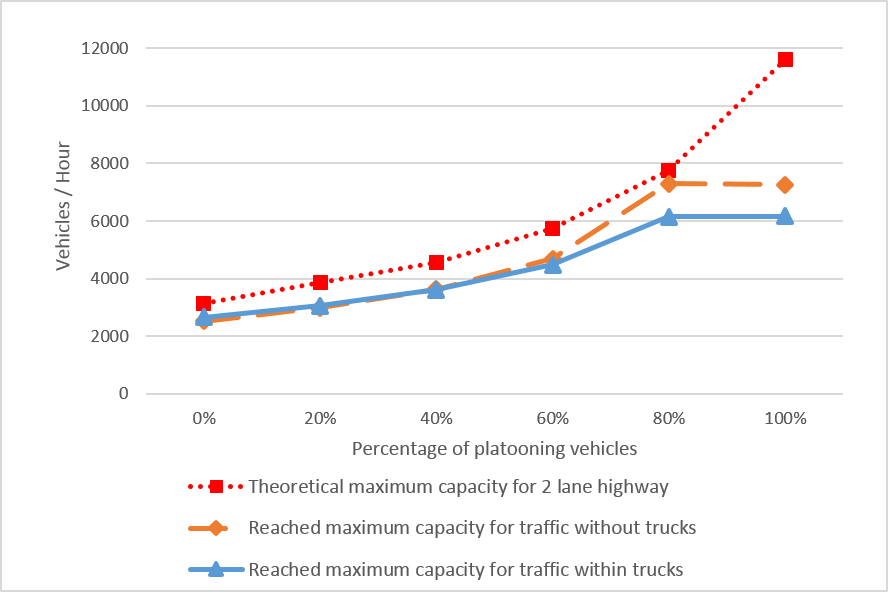
\includegraphics[width=0.82\textwidth,height=0.82\textheight,keepaspectratio]{figures/Chapter_5/5_E3_maxCap.png}
\centering
\protect\caption[Maximum capacity of two-lane highway of Theoretical example, real traffic without truck and real traffic with trucks]{\label{fig:5_3-4}Maximum capacity of two-lane highway of Theoretical example, real traffic without truck and real traffic with trucks - capacity measured only for 0\%, 20\%, 40\%, 60\%, 80\%, 100\% platooning vehicles, so as to be more visual the line connecting measured data was added.}
\end{figure}

The effect of vehicle \textit{speed dispersion} results in a reduction of efficiency of platooning concept. It is caused by slowing down of each lane by the slower vehicles. Truck traffic also negatively effects the effectiveness of platooning on maximum capacity. The reason of that is the composition of traffic, 35\% of all traffic are trucks which occupy the slowest lane and their maximum speed is 25 m/s. It can be said they make the lane unusable for platoons of passenger vehicles.














\section[Experiment \#4: Maximum capacity of three-lane highway with real traffic conditions of the Czech Republic]{Experiment \#4: Maximum capacity of three-lane highway with real traffic conditions of the Czech Republic\sectionmark{Experiment \#4...}}
\sectionmark{Experiment \#4...}

This experiment is very similar to Experiment \#3. With the same conditions we run the simulation of highway of length 5 km for 15 minutes to find out, how the traffic would behave for different percentage of platooning vehicles. 

We expected that, according to the results from Experiment \#2 and the table \ref{tab:5_2-1}, the maximum capacity of three-lane highway with traffic without trucks is proportionally smaller than theoretical maximum capacity. But for traffic with trucks we expected increasing of maximum capacity. According to 35\% representation of trucks in the traffic, the lane on the very right serves for  truck traffic and the other  two left lanes can be fully used for platooning passenger vehicles.



\subsection*{Simulator setting for the test}
\begin{itemize}
\item Average speed: 34 m/s
\item Speed dispersion: 3 m/s
\item Length of platoon: 2-6
\item Number of lanes:  3
\item Platooning vehicles ratio: 0\%, 20\%, 40\%, 60\%, 80\%, 100\%
\item Generation limit: false
\item Generate trucks: false, true
\item Percentage of passenger vehicles in traffic: 65\%
\item Overtaking: Snake type
\end{itemize}



\subsection*{Experiment results}
We did simulations with traffic in three-lane highway without truck traffic (see maximum reached capacity during time in Figure \ref{fig:5_4-1}) and with included truck traffic (See level of maximum reached capacity during time in Figure \ref{fig:5_4-2}). The simulations show very similar trend of results such as Experiment \#3.


\begin{figure}[ph]
\centering
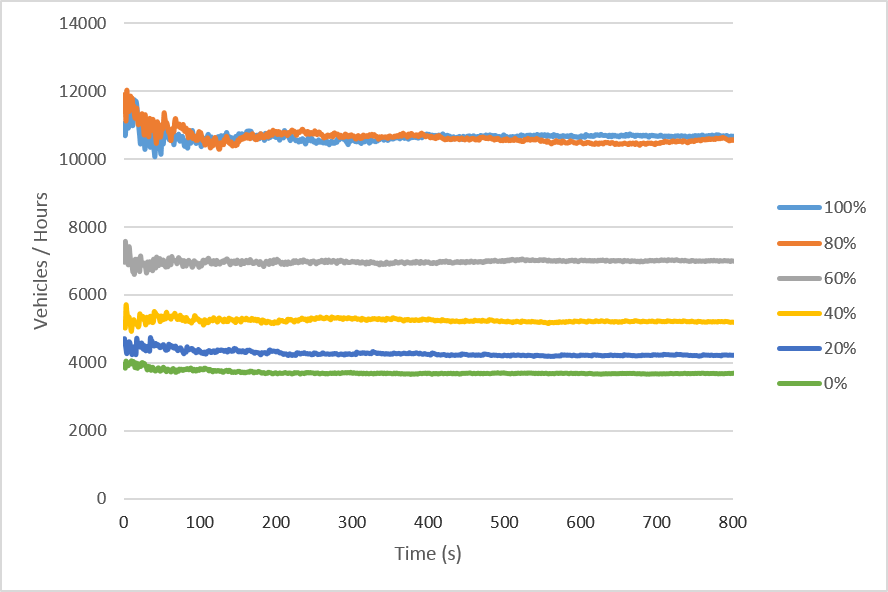
\includegraphics[width=0.82\textwidth,height=0.82\textheight,keepaspectratio]{figures/Chapter_5/5_3l_NT_maxCap.png}
\centering
\protect\caption[Maximum capacity of three-lane highway and real traffic conditions without trucks]{\label{fig:5_4-1}Maximum capacity of three-lane highway and real traffic conditions without trucks}
\end{figure}

\begin{figure}[ph]
\centering
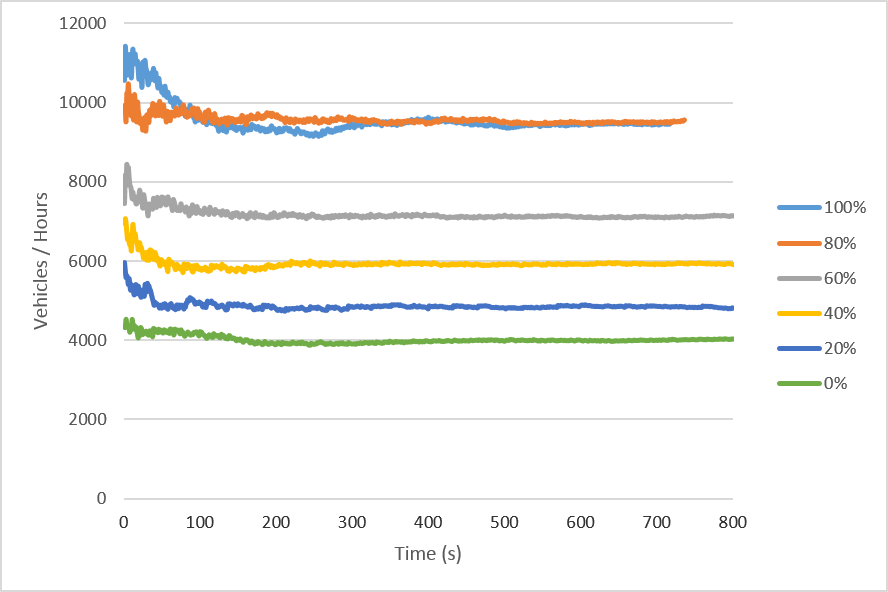
\includegraphics[width=0.82\textwidth,height=0.82\textheight,keepaspectratio]{figures/Chapter_5/5_3l_T_maxCap.png}
\centering
\protect\caption[Maximum capacity of three-lane highway and real traffic conditions with trucks]{\label{fig:5_4-2}Maximum capacity of three-lane highway and real traffic conditions with trucks}
\end{figure}


Comparison of ratio between theoretical maximum values and our reached ones in Table \ref{tab:5_4-1} and Table \ref{tab:5_3-1} of previous Experiment \#3 showed that platooning has positive effect on traffic with trucks in three-lane highway and traffic without trucks in two-lane highway. We could see during each simulation that the slowest lane of three-lane highway was used only for truck traffic.

\begin{table}[ph]
\begin{centering}
\begin{tabular}{|c|c|c|c|c|c|c|}
\hline 
 ... / Platooning \% &	0\% &	20\% &	40\% &	60\% &	80\% &	100\%\tabularnewline
\hline 
Theoretical maximum &	4 725 &	5 793 &	6 840 &	8622 &	11 634 &	17 433
\tabularnewline
 capacity for 3 lane highway & & & & & &\tabularnewline
\hline 
Reached maximum capacity & 3 661 &	4 230 &	5 219 &	6 993 &	10 478 &	10 677
\tabularnewline
for traffic without trucks & & & & & &\tabularnewline
\hline 
Ratio Theoretical maximum & & & & & &\tabularnewline
capacity / Reached maximum & 77.49\% &	73.01\% &	76.30\% &	81.11\% &	90.06\% &	61.24\%\tabularnewline
capacity without trucks & & & & & &\tabularnewline
\hline 
Reached maximum capacity & 4 001 &	4 845 &	5 920 &	7 108 &	9 501 &	9 448\tabularnewline
for traffic with trucks & & & & & &\tabularnewline
\hline 
Ratio Theoretical maximum & & & & & &\tabularnewline
capacity / Reached maximum & 84.68\% &	83.63\% &	86.56\% &	82.43\% &	81.67\% &	54.20\%\tabularnewline
capacity with trucks & & & & & &\tabularnewline
\hline 
\end{tabular}
\centering
\protect\caption{\label{tab:5_4-1}Reached maximum capacities of three-lane highway and their comparison to theoretical maximum 3 lane highway}
\end{centering}
\end{table}

\begin{figure}[ph]
\centering
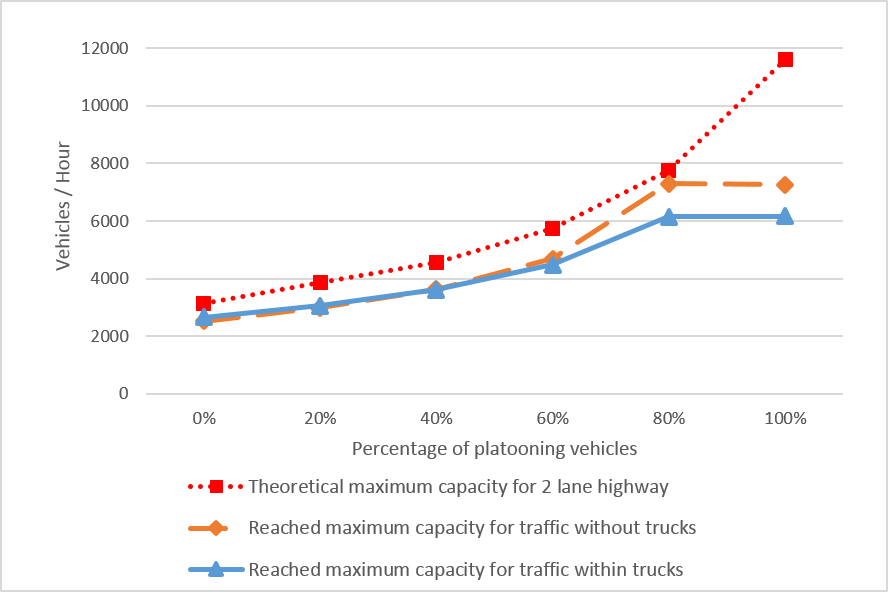
\includegraphics[width=0.82\textwidth,height=0.82\textheight,keepaspectratio]{figures/Chapter_5/5_2lane_maxCap.png}
\centering
\protect\caption[Maximum capacity of three-lane highway of Theoretical example, real traffic without truck and real traffic with trucks]{\label{fig:5_4-3}Maximum capacity of three-lane highway of Theoretical example, real traffic without truck and real traffic with trucks - capacity measured only for 0\%, 20\%, 40\%, 60\%, 80\%, 100\% platooning vehicles, so as to be more visual the line connecting measured data was added.}
\end{figure}

We measured average speed of passenger vehicles which can be seen in Figure \ref{fig:5_4-4}. Both experiments \#3 and \#4 show the relation between percentage of platooning vehicles and average speed in maximum usage of highway.  There is trend, that with increasing percentage of platooning vehicles the average speed is decreasing in time. The reason of that is studied in next Chapter 6.

\begin{figure}[!htbp]
\centering
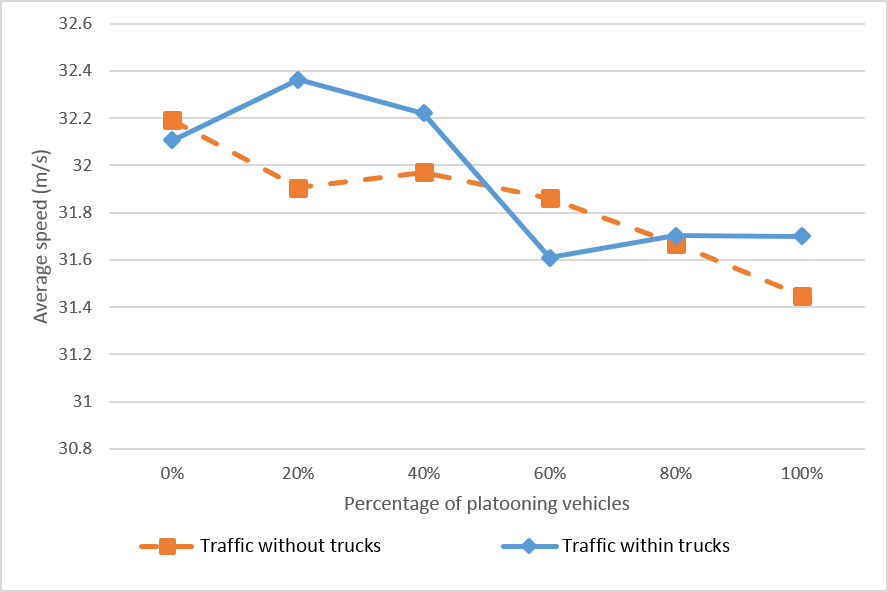
\includegraphics[width=0.82\textwidth,height=0.82\textheight,keepaspectratio]{figures/Chapter_5/5_E4_averageSpeed.png}
\centering
\protect\caption[Average speed of traffic without and with trucks in three-lane highway]{\label{fig:5_4-4}Average speed of traffic without and with trucks in three-lane highway - average speed measured after stabilization of traffic and only for 0\%, 20\%, 40\%, 60\%, 80\%, 100\% platooning vehicles, so as to be more visual the line connecting measured data was added.}
\end{figure}















\newpage
\section[Experiment \#5: Effect of platooning concept on Traffic model \#1 ]{Experiment \#5: Effect of platooning concept on Traffic model \#1\sectionmark{Experiment \#5...}}
\sectionmark{Experiment \#5...}

We used platooning concept on real traffic situation of Czech highway. The experiment setting is based on parameters of traffic model \#1 in Chapter 2 (three-lane highway). Based on information from previous Experiment \#4 we knew that maximum capacity of three-lane highway without platooning concept is cca 3700 vehicles per hour (Table \ref{tab:5_4-1}). Traffic model \#1 supposes density of vehicles 3200 vehicles per hour, so we can expect that platoons make the highway more „open“ and could increase average speed of passenger vehicles.

We also wanted to see how the platooning concept influences the traffic model \#1 with double level of traffic density, 6400 vehicles per hour. Based on the previous experiments, we knew that this capacity cannot be reached without higher level of percentage of platoon vehicles.



\subsection*{Simulator setting for the test}

Settings of Traffic model \#1.
\begin{itemize}
\item Average speed: 34 m/s
\item Speed dispersion: 3 m/s
\item Length of platoon: 2-6
\item Number of lanes:  3
\item Platooning vehicles ratio: 0\%, 20\%, 40\%, 60\%, 80\%, 100\%
\item Generation limit: 3200 vehicles / hour, 6400 vehicles / hour
\item Generate trucks: true
\item Percentage of passenger vehicles in traffic: 67\%
\item Overtaking: Snake type
\end{itemize}




\subsection*{Experiment results}

From this test which corresponds to traffic model \#1 and from the Figure \ref{fig:5_5-1} we could see that average speed of passenger vehicles is reduced to level 32.8 m/s for 0\% platooning vehicles . It is caused by high density of vehicles which is close to the maximum capacity of three-lane highway. And for for 100\% platooning vehicles the average speed reached value  34.3 m/s. The Figure \ref{fig:5_5-1} also shows a positive effect of platooning on average speed in simulated situation based on real traffic parameters.

We also simulated Traffic model \#1 with double traffic. The desired traffic density was reached between 40\% and 60\% platooning vehicles as can be seen in Figure \ref{fig:5_5-2}. In Figure \ref{fig:5_5-1} the positive effect of platooning on average speed can be also seen.




\begin{figure}[ht]
\centering
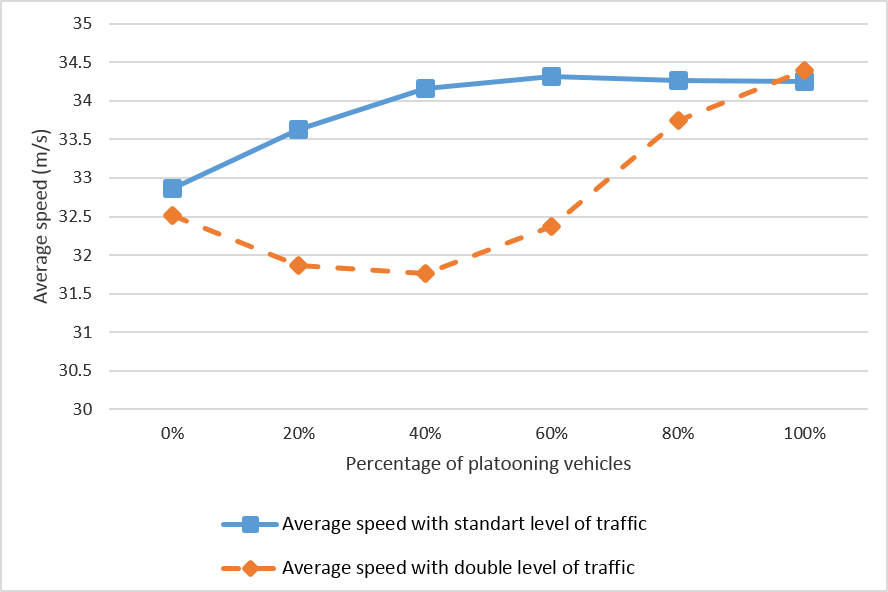
\includegraphics[width=0.82\textwidth,height=0.80\textheight,keepaspectratio]{figures/Chapter_5/5_M1_avgSpeed.png}
\centering
\protect\caption[Average speed of Traffic model \#1 with standard and double level of traffic]{\label{fig:5_5-1}Average speed of Traffic model \#1 with standard and double level of traffic - average speed measured after stabilization of traffic and only for 0\%, 20\%, 40\%, 60\%, 80\%, 100\% plat. vehicles, so as to be more visual the line connecting meas. data was added.}
\end{figure}


\begin{figure}[!htbp]
\centering
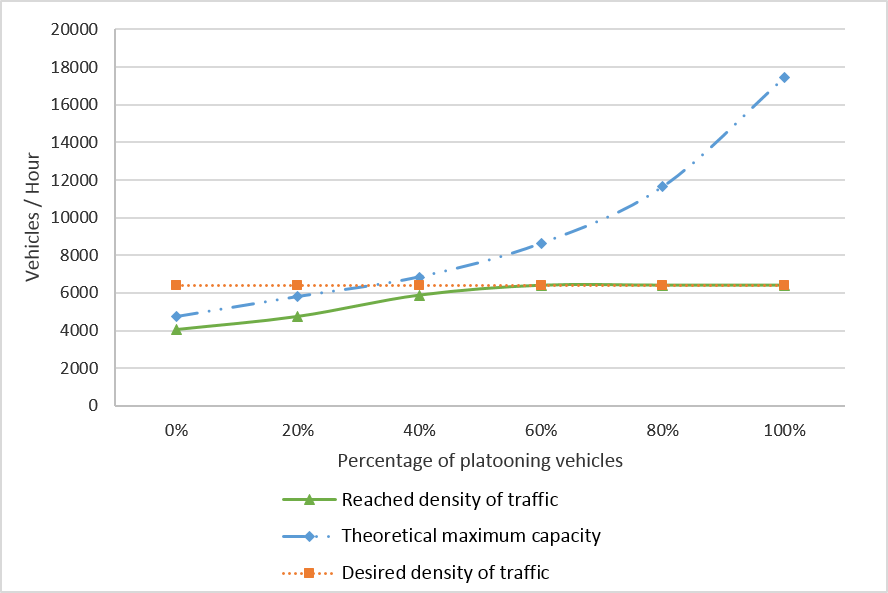
\includegraphics[width=0.82\textwidth,height=0.80\textheight,keepaspectratio]{figures/Chapter_5/5_M1D_cap.png}
\centering
\protect\caption[Reached density of Traffic model \#1 with double level of traffic for  percentage of platooning vehicles]{\label{fig:5_5-2}Reached density of Traffic model \#1 with double level of traffic for percentage of platooning vehicles - traffic density measured only for 0\%, 20\%, 40\%, 60\%, 80\%, 100\% platooning vehicles, so as to be more visual the line connecting measured data was added.}
\end{figure}

















\newpage
\section[Experiment \#6: Effect of platooning concept on Traffic Model \#2]{Experiment \#6: Effect of platooning concept on Traffic Model \#2\sectionmark{Experiment \#6...}}
\sectionmark{Experiment \#6...}


This experiment had the same assumption as Experiment \#5 but only for Traffic model \#2 (two- lane highway).



\subsection*{Simulator setting for the test}
Settings of Traffic model \#2.
\begin{itemize}
\item Average speed: 34 m/s
\item Speed dispersion: 3 m/s
\item Length of platoon: 2-6
\item Number of lanes:  2
\item Platooning vehicles ratio: 0\%, 20\%, 40\%, 60\%, 80\%, 100\%
\item Generation limit: 1650 vehicles / hour, 3300 vehicles / hour
\item Generate trucks: true
\item Percentage of passenger vehicles in traffic: 67\%
\item Overtaking: Snake type
\end{itemize}



\subsection*{Experiment results}

From this experiment of standard Traffic model \#2, in the Figure \ref{fig:5_6-1}, we could see that average speed of passenger vehicles is reduced to level 33.2 m/s for 0\% platooning vehicles. It is higher  average speed than we could see in Experiment \#5, the Figure \ref{fig:5_5-1}, but this test is two-lane highway and Experiment \#5 was three-lane highway . The Figure \ref{fig:5_6-1} also shows again a positive effect of platooning on average speed in real situation. Value of average speed is increasing with percentage of platooning vehicles, with 100\% the value with higher than 34 m/s.

Double of the capacity of Traffic model \#2 was reached between 20\% and 40\% platooning vehicles and  in Figure \ref{fig:5_6-2}  the positive effect of platooning on average speed can be also seen.


\begin{figure}[ph]
\centering
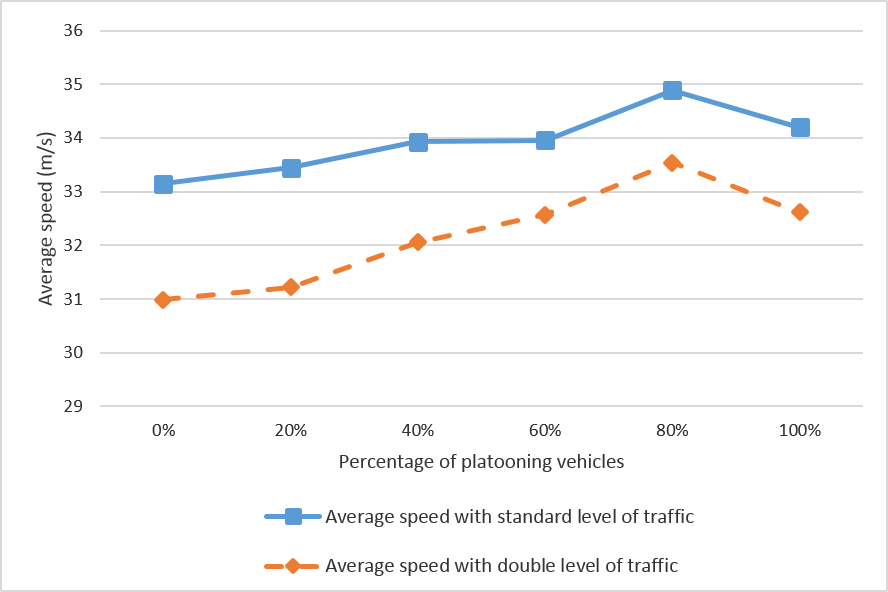
\includegraphics[width=0.82\textwidth,height=0.80\textheight,keepaspectratio]{figures/Chapter_5/5_M2_avgSpeed.png}
\centering
\protect\caption[Average speed of Traffic model \#2 with standard and double level of traffic]{\label{fig:5_6-1}Average speed of Traffic model \#2 with standard and double level of traffic - average speed measured after stabilization of traffic and only for 0\%, 20\%, 40\%, 60\%, 80\%, 100\% platooning vehicles, so as to be more visual the line connecting measured data was added.}
\end{figure}


\begin{figure}[ph]
\centering
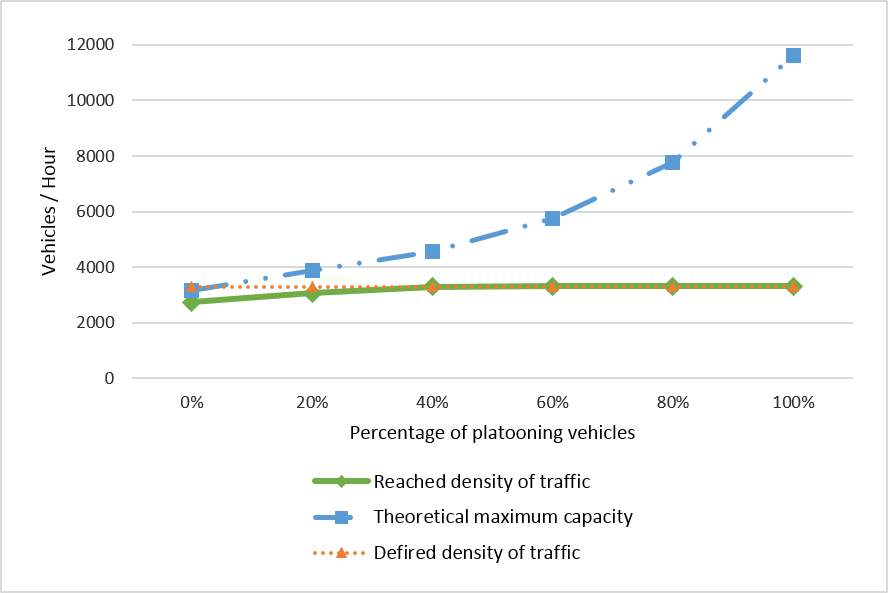
\includegraphics[width=0.82\textwidth,height=0.80\textheight,keepaspectratio]{figures/Chapter_5/5_M2D_cap.png}
\centering
\protect\caption[Reached density of Traffic model \#2 with double level of traffic for  percentage of platooning vehicles]{\label{fig:5_6-2}Reached density of Traffic model \#2 with double level of traffic for  percentage of platooning vehicles - traffic density measured only for 0\%, 20\%, 40\%, 60\%, 80\%, 100\% platooning vehicles, so as to be more visual the line connecting measured data was added.}
\end{figure}